\subsection{Architecture}

In figure \ref{fig:architecture} is shown a simple diagram of the architecture used from both the Android and Desktop application. We used the \textit{Event Bus} architectural pattern in order to obtain high decoupling between all the modules.

\begin{figure}[htbp]
	\centering
	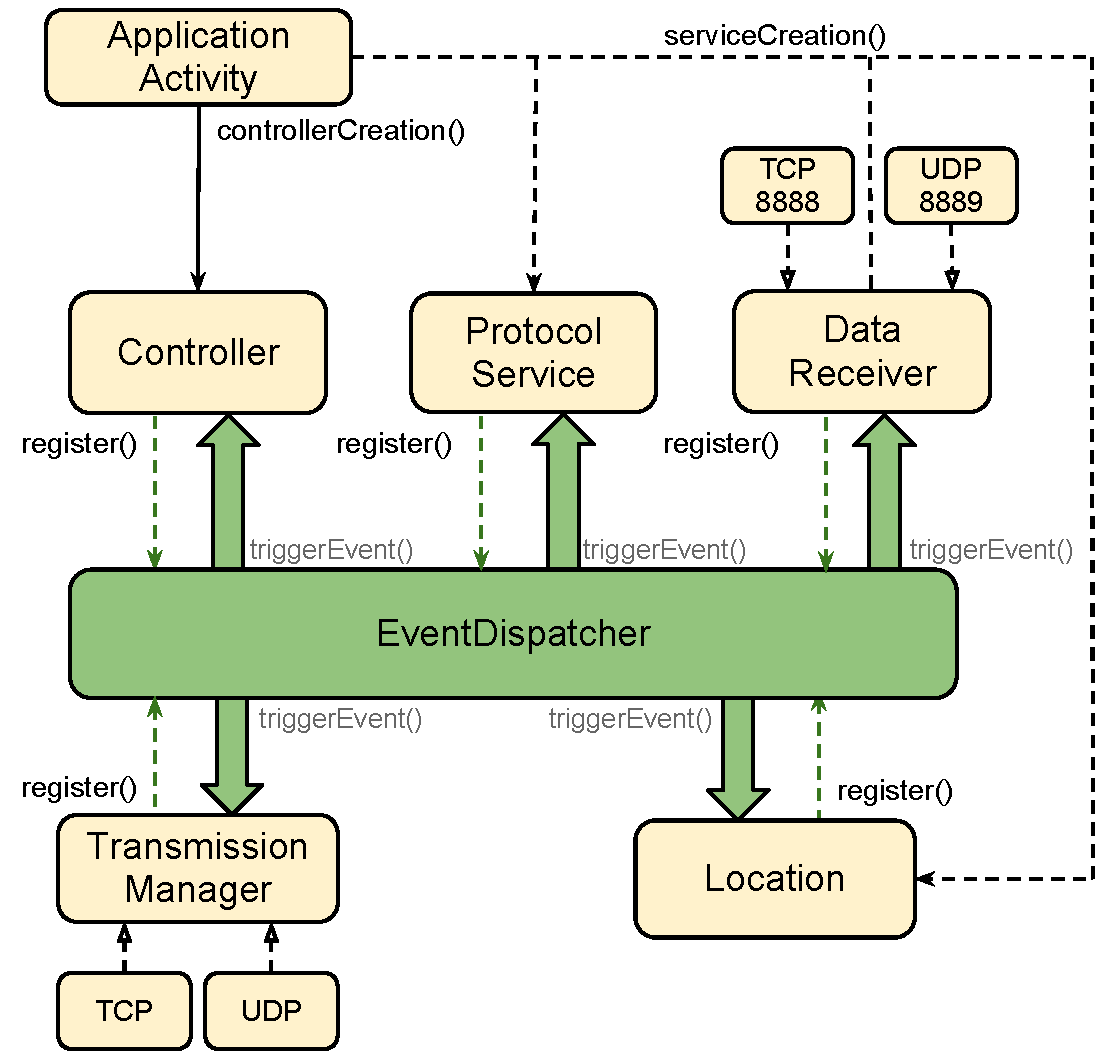
\includegraphics[trim = 10mm 0mm 0mm 0mm,width=3.5in]{imgs/components_architecture.pdf}
	\caption{Graphical representation of application structure.}
	\label{fig:architecture}
\end{figure}

Given this architecture, changing or adding new modules is as easy as registering them within the \textit{Event Bus} as \textit{Components} listening for needed events. It's worth mentioning that the desktop application uses only one type of transmission (raw data link layer packets), while the Android applications can only use TCP or UDP because of system limitations.

